\documentclass[14pt,fleqn]{extarticle}
\RequirePackage{prepwell-eng}

\previewoff 

\begin{document} 
\begin{skill}
    \begin{narrow}
\textcolor{blue}{Circle Basics} 
 
    \end{narrow}
    
    \reason 
    
    \begin{center}
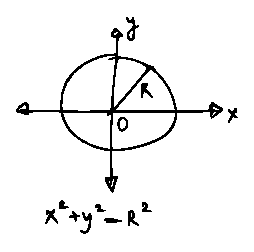
\includegraphics[scale=1.5]{circle.eps} 
\end{center} 

A circle is the locus of all points that are equi-distant from a given point (known as the center) \newline 

The figure above shows a circle whose center is at the origin $O$\newline 

It does not have to be though. The center can be at any point $(a,b)$\newline 

The \underline{standard equation} of a circle with center at $(a,b)$ and radius $R$   is 
\[ \qquad \left(x-a \right)^2 + \left(y-b \right)^2 = R^2 \]

When the center is at the origin, that is $(a,b) = (0,0)$, then this boils down to 
\[ \qquad x^2 + y^2 = R^2 \]
\end{skill}

\end{document} 